\documentclass{article}
\usepackage[top=1in, bottom=1in, left=1in, right=1in]{geometry}
\usepackage{polski}
\usepackage[utf8]{inputenc}
\usepackage{graphicx}
\begin{document}
\title{\huge\bfseries Wyznaczanie przyspieszenia ziemskiego za pomocą wahadła rewersyjnego}
\date{}
\author{}
\maketitle
\section{Wstęp teoretyczny}
\subsection{Siła grawitacji}
Siła Grawitacji czyli siła ciążenia powszechnego jest zjawiskiem naturalnym, polegającym na oddziaływaniu na siebie, wzajemnie przyciągając się,  wszystkich obiektów które posiadają masę.\\\\
	Opierając sie na zależności siły grawitacyjnej, możemy obliczyć siłę $F_g$ z jaką planeta oddziałowuje na ciało o masie $m$:
	$$F_g = \frac{GM_zm}{{r_z^2}}$$
	 \begin{center}
	 $M_z \approx 5,9736 * 10^{24}$ kg - masa Ziemi, $r_z \approx 6373,14$km
	 \end{center}
\subsection{Przyspieszenie ziemskie, jednostka, zależność wartości od szerokości geograficznej i wysokości nad poziomem morza}
Przyspieszenie ziemskie - g jest to przyspieszenie grawitacyjne działająca na ciała swobodnie spadające na Ziemię(pomijając opory ruchów). 
$$g = \frac{GM_z}{r^2} \approx \frac{6,6732 \cdot 10^{-11} \cdot m^3\cdot kg^{-1}\cdot s-2 \cdot 5,9736 \cdot 10^{24}kg}{(6373,14km)^2} \approx 9,81 \frac{m}{s^2}$$
$$[g] = \frac{N}{kg} = \frac{m}{s^2}$$
Wartość przyspieszenia ziemskiego jest zależna od szerokości geograficznej oraz od wysokości nad poziomem morza. Przy wzroście wysokości, zwiększa się odległość od środka Ziemi, przez co przyspieszenie ziemskie maleje.\\
Wpływ na przyspieszenie ziemskie spowodowane szerokością geograficzną wynika z ruchu obrotowego Ziemi - na ciało znajdujące się na powierzchni planety działa siła odśrodkowa o przeciwnym zwrocie do siły grawitacji, przez co obserwujemy dany spadek wartości.
\subsection{Wahadło matematyczne oraz zależność okresu drgań od długości jego wahadła}
Idealnym wahadłem matematycznym możemy nazwać punktową masę m, zawieszoną na nieważkiej i nierozciągliwej linie. W praktyce, przybliżonym tworem jest niewielka metalowa kulka zawieszona na mocnej nitce. Okres drgań wahadła nie zależy od masy m tylko od długości wahadła l i dla małych kątów wynosi:
$$T = 2\pi \sqrt\frac{l}{g}$$
\subsection{Wahadło fizyczne i rewersyjne }
Wahadło fizyczne jest to ciało wykonujące wahania wokół poziomej osi obrotu nie przechodzącej przez środek masy ciała. Wahadłem fizycznym o dwóch równoległych osiach zawieszenia i regulowanym rozkładzie masy nazywamy wahadłem rewersyjnym. Dzięki temu możliwe jest osiągnięcie identyczności okresu drgań przy obu sposobach zawieszenia.\\\\
Długość zredukowana wahadła rewersyjnego to taka długość wahadła matematycznego dla której okres drgań jest taki sam jak dla wahadła fizycznego. Długość zredukowana wyraża się wzorem:
$$L=\frac{i}{md}$$
gdzie:\\

$l$ - długość wahadła

$m$ - masa wahadła

$i$ -moment bezwładności

$d$ - odległość środka masy od osi obrotu\\\\
Odwracalność wahadła rewersyjnego to własność wahadła fizycznego, która sprawia, że jego zachowanie jest bardzo zbliżone do zachowania wahadła matematycznego.
\begin{flushright}
\begin{scriptsize}
Źródła: \textit{http://www.fizykon.org/grawitacja/grawitacja$\_$wprowadzenie.htm} \\
\textit{http://pl.wikipedia.org/wiki/Grawitacja}\\
\textit{http://pl.wikipedia.org/wiki/Przyspieszenie$\_$ziemskie}\\
\textit{https://pl.wikipedia.org/wiki/Wahadło\_rewersyjne}\\
\end{scriptsize}
\end{flushright}
\section{Przebieg i cel ćwiczenia}
Celem ćwiczenia jest wyznaczenie przyspieszenia ziemskiego przy pomocy wahadła rewersyjnego. Stanowisko pomiarowe składa się ze skali centymetrowej oraz zawieszonego nad nią wahadła matematycznego oraz rewersyjnego, które składa się z pręta , na którym umieszczone są dwa obciążniki. Poprzez regulowanie położenia elementu ruchomego(ruchomej masy - obciążnika) zmieniamy położenie środka masy wahadła. Każde wahnięcie, mierzone jest za pomocą fotokomórki. Mierzymy czas 10 wahnięć z początkowym położeniem masy równej $2cm$, przesuwamy masę o $2cm$, aż do osiągnięcia końca miary - $42cm$. Następnie obracamy wahadło i powtarzamy pomiary. Po ustaleniu i ustawieniu położenia odwracalnego wahadła, mierzymy czas wykonania 100 pełnych wahnięć przed i po odwróceniu.
\subsection{Opracowanie pomiarów}
Pomiary zostały przedstawione w następującej tabeli:
\begin{center}
    \begin{tabular}{|c|c|c|c|c|c|c|}
    \hline
    \multicolumn{3}{|c|}{$l[cm]$} & \multicolumn{4}{|c|}{$2cm-42cm$} \\ \hline
    \multicolumn{3}{|c|}{Liczba okresów $N$} & \multicolumn{4}{|c|}{$10$} \\ \hline
    Lp. & $x[cm]$ & $x[m]$ & $t_1[s]$ & $t_2[s]$ & $T_1[s]$ & $T_2[s]$\\ \hline
    1 & $2$ & $0,02$ & $13,37$ & $13,26$ & $1,337$ & $1,326$ \\ \hline
2 & $4$ & $0,04$ & $11,93$ & $13,08$ & $1,193$ & $1,308$ \\ \hline
3 & $6$ & $0,06$ & $11,18$ & $12,92$ & $1,118$ & $1,292$ \\ \hline
4 & $8$ & $0,08$ & $10,72$ & $12,75$ & $1,072$ & $1,275$ \\ \hline
5 & $10$ & $0,1$ & $10,46$ & $12,69$ & $1,046$ & $1,269$ \\ \hline
6 & $12$ & $0,12$ & $10,36$ & $12,62$ & $1,036$ & $1,262$ \\ \hline
7 & $14$ & $0,14$ & $10,36$ & $12,56$ & $1,036$ & $1,256$ \\ \hline
8 & $16$ & $0,16$ & $10,43$ & $12,52$ & $1,043$ & $1,252$ \\ \hline
9 & $18$ & $0,18$ & $10,55$ & $12,51$ & $1,055$ & $1,251$ \\ \hline
10 & $20$ & $0,2$ & $10,73$ & $12,5$ & $1,073$ & $1,25$ \\ \hline
11 & $22$ & $0,22$ & $10,91$ & $12,54$ & $1,091$ & $1,254$ \\ \hline
12 & $24$ & $0,24$ & $11,13$ & $12,57$ & $1,113$ & $1,257$ \\ \hline
13 & $26$ & $0,26$ & $11,37$ & $12,62$ & $1,137$ & $1,262$ \\ \hline
14 & $28$ & $0,28$ & $11,6$ & $12,68$ & $1,16$ & $1,268$ \\ \hline
15 & $30$ & $0,3$ & $11,86$ & $12,75$ & $1,186$ & $1,275$ \\ \hline
16 & $32$ & $0,32$ & $12,11$ & $12,84$ & $1,211$ & $1,284$ \\ \hline
17 & $34$ & $0,34$ & $12,37$ & $12,93$ & $1,237$ & $1,293$ \\ \hline
18 & $36$ & $0,36$ & $12,62$ & $13,03$ & $1,262$ & $1,303$ \\ \hline
19 & $38$ & $0,38$ & $12,87$ & $13,13$ & $1,287$ & $1,313$ \\ \hline
20 & $40$ & $0,4$ & $13,13$ & $13,25$ & $1,313$ & $1,325$ \\ \hline
21 & $42$ & $0,42$ & $13,39$ & $13,39$ & $1,339$ & $1,339$ \\ \hline
    \end{tabular}
\end{center}
Oraz dla stu wahnięć:
\begin{center}
    \begin{tabular}{|c|c|c|c|c|c|c|}
    \hline
    \multicolumn{3}{|c|}{$l[cm]$} & \multicolumn{4}{|c|}{$42cm$} \\ \hline
    \multicolumn{3}{|c|}{Liczba okresów $N$} & \multicolumn{4}{|c|}{$100$} \\ \hline
    Lp. & $x[cm]$ & $x[m]$ & $t_1[s]$ & $t_2[s]$ & $T_1[s]$ & $T_2[s]$\\ \hline
    1 & $42$ & $0,42$ & $133,78$ & $134,34$ & $1,338$ & $1,343$ \\ \hline
    \end{tabular}
\end{center}
Położenie odwracalne wahadła ustalone zostało na długości $l = 42cm$. Obliczając za pomocą wzoru 
$$T = \frac{t}{N}$$
okres drgań gdzie $t$ to zmierzony czas, a $N$ to ilość wahnięć, przedstawiał się następująco:
\begin{center}
    \begin{tabular}{|c|c|c|c|c|}
    \hline
    $l$ & $T_1[s]$ & $T_2[s]$ & $T_3[s]$ & $T_4[s]$ \\ \hline
    $0,42$ & $1,339$ & $1,339$ & $1,338$ & $1,343$ \\ \hline
    
    \end{tabular}
\end{center}
Aby obliczyć niepewność pomiaru czasu $u(t)$  oraz okresów drgań $u(T)$ zastosowaliśmy wzór
$$u(t) = \sqrt{\frac{\Sigma(t_i-\overline{t})^2}{n(n-1)}}$$
gdzie, $n=4$.
$$t = 13,4045s,\ u(t) = 0,0128949s$$
\begin{center}
oraz
\end{center}
$$T = 1,34045s,\ u(T) = 0,0012895s$$
więc 
$$T = 1,34045\pm 0,0012895 s$$
Niepewność rozszerzoną obliczamy ze wzoru:
$$U(T)=k\cdot u(T)$$
, gdzie k to współczynnik rozszerzenia równy $2$.
$$U(T)=2\cdot u(T)=2\cdot 0,0012895=0,002579s$$
Opierając się na wzorze na okres drgań wahadła matematycznego,
$$g = \frac{4\pi^2l}{T^2}$$
obliczamy wartość przyspieszenia ziemskiego $g$ dla okresu drgań wahadła rewersyjnego w położeniu odwracalnym i wynosi ono około
$$g\approx9,667367\frac{m}{s^2}$$
następnie w oparciu o prawo przenoszenia niepewności, obliczamy niepewność wyznaczonej wartości $g$
$$u_c(g) = \frac{4\pi^2l}{2T}\cdot u(T) = 0,0083551 \frac{m}{s^2}$$
oraz jej niepewność rozszerzoną
$$U(g) = 0,01671019\frac{m}{s^2}$$
Aby obliczyć przyspieszenie ziemskie dla szerokości geograficznej oraz wysokości nad poziomem morza Gliwic potrzebowaliśmy danych, które wynoszą $h=240 m.n.p.m.$ oraz $\varphi = 50,31^{\circ}$. Podstawiając wartości do wzoru:
$$g\approx 9780318(1+0,0053024\sin^2 \varphi-0,0000058\sin^2 2\varphi ) - 3,086\cdot 10^{-6}h \approx 9,7796 \frac{m}{s^2}$$
\subsection{Wnioski}
Otrzymane wyniki odbiegają od siebie o około $0,1\frac{m}{s^2}$, więc można określić je jako zbliżone. Różnica wynikać może z niedokładności sprzętu pomiarowego oraz opóźnienia związanego z ludzką reakcją, gdyż przy mierzeniu stu wahnięć, stoper nie zatrzymywał się przez co wymagał ręcznego zatrzymania. 

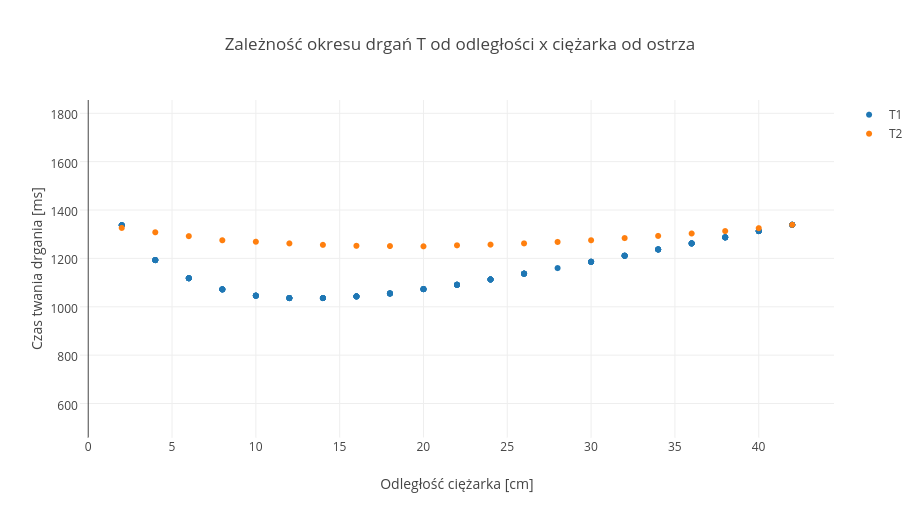
\includegraphics[height=0.6\textheight, angle =90]{Plot2.png}
\end{document}